\documentclass[border=4pt]{standalone}
\usepackage[T1]{fontenc}
\usepackage{helvet}
\renewcommand{\familydefault}{\sfdefault}
\usepackage{graphicx}
\usepackage{caption}
\usepackage{amsmath}
\captionsetup{font={sf,footnotesize},labelfont={sf,bf,footnotesize},justification=justified,singlelinecheck=false}
\begin{document}
\setcounter{figure}{16}
\begin{minipage}{7.20in}
\centering
\begin{figure}[htbp]
    \centering
    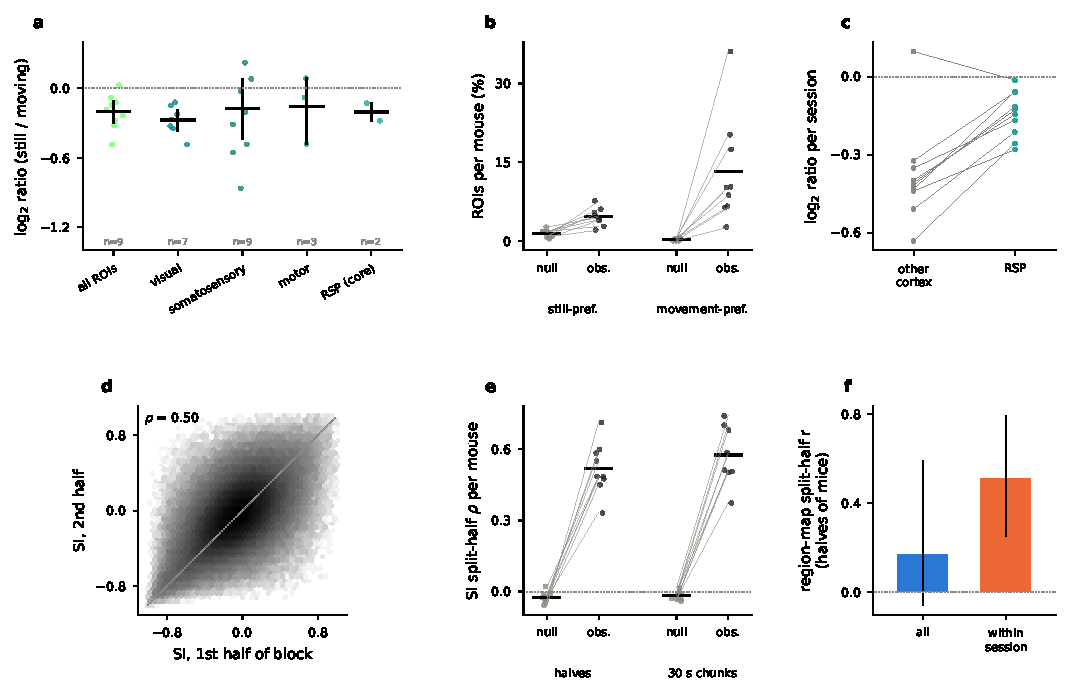
\includegraphics[width=\linewidth]{fig17_meso_still_panels.pdf}
    \caption{Correlates of stillness in the IBL mesoscope: lower activity in stillness across dorsal cortex. \textbf{a} Activity in still against moving 1\,s bins of the passive block before the task replay (grey screen and receptive-field mapping; median 6.2\,min per session), log$_2$((still\,+\,$e$)/(moving\,+\,$e$)) of each ROI's deconvolved activity with $e$ = 2\% of its mean; ROIs averaged per session (sessions with $\geq$20 ROIs in the group), sessions per mouse. Moving: lick or face motion energy above the session's 60th percentile (the wheel is not recorded in this block); still: no movement within $\pm$1\,s and $\leq$30\,s after the last movement. Groups by Beryl region (Allen colours); black, mean and 95\% bootstrap CI over mice; n, mice. \textbf{b} Still- and movement-preferring ROIs per mouse (Welch test of still against moving bins, at most one of each per 2\,s, $p<0.01$), observed against a circular-shift null (activity rotated against the behavioural labels, 100 offsets $\geq$60\,s). Bars: means over mice. One session whose null exceeded 5\% (slow drift; a quarter of its ROIs silent in all still bins) is excluded from all panels. \textbf{c} RSP against the other imaged ROIs of the same session (lines: sessions).}
    \label{fig:meso_still}
\end{figure}
\end{minipage}
\end{document}
